% Fig 3.3 — BM25S indexing flow
\documentclass[border=4pt]{standalone}
\usepackage{tikz}
\usetikzlibrary{positioning, arrows.meta, shapes.geometric}
\begin{document}
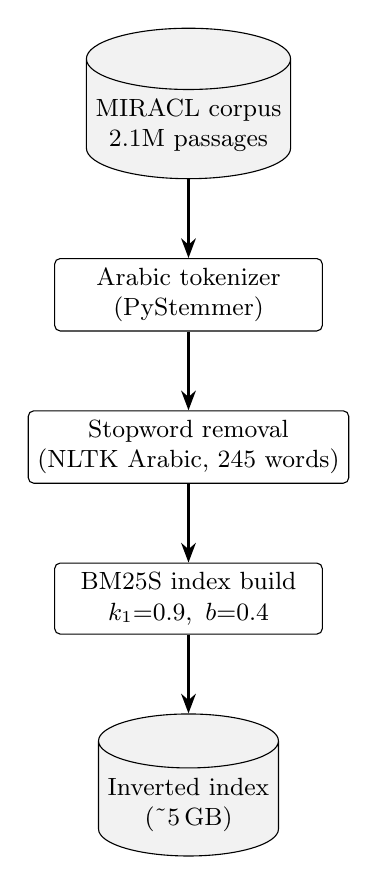
\begin{tikzpicture}[
    >=Stealth, node distance=10mm,
    box/.style={rectangle, draw, rounded corners=2pt,
                minimum width=34mm, minimum height=9mm,
                align=center, font=\small},
    data/.style={cylinder, shape border rotate=90, aspect=0.3,
                 draw, minimum width=22mm, minimum height=10mm,
                 align=center, font=\small, fill=black!5},
    arrow/.style={-{Stealth[length=2.5mm]}, thick}
]
  \node[data] (corpus) {MIRACL corpus\\2.1M passages};
  \node[box, below=of corpus] (tok) {Arabic tokenizer\\(PyStemmer)};
  \node[box, below=of tok] (stop) {Stopword removal\\(NLTK Arabic, 245 words)};
  \node[box, below=of stop] (idx) {BM25S index build\\$k_1{=}0.9,\ b{=}0.4$};
  \node[data, below=of idx] (index) {Inverted index\\(\textasciitilde 5\,GB)};

  \draw[arrow] (corpus) -- (tok);
  \draw[arrow] (tok) -- (stop);
  \draw[arrow] (stop) -- (idx);
  \draw[arrow] (idx) -- (index);
\end{tikzpicture}
\end{document}
